

\tikzset{every picture/.style={line width=0.75pt}} %set default line width to 0.75pt        

%
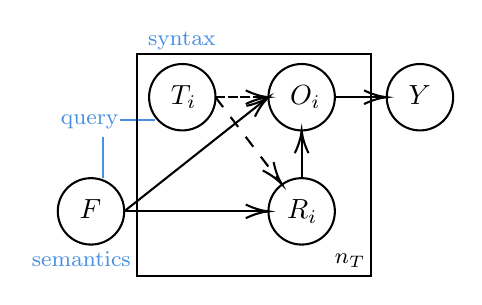
\begin{tikzpicture}[x=0.75pt,y=0.75pt,yscale=-1,xscale=1]
%uncomment if require: \path (0,300); %set diagram left start at 0, and has height of 300

%Shape: Circle [id:dp03401517896749362] 
\draw   (222,116) .. controls (222,107.16) and (229.16,100) .. (238,100) .. controls (246.84,100) and (254,107.16) .. (254,116) .. controls (254,124.84) and (246.84,132) .. (238,132) .. controls (229.16,132) and (222,124.84) .. (222,116) -- cycle ;
%Shape: Circle [id:dp413585029775966] 
\draw   (279.5,116) .. controls (279.5,107.16) and (286.66,100) .. (295.5,100) .. controls (304.34,100) and (311.5,107.16) .. (311.5,116) .. controls (311.5,124.84) and (304.34,132) .. (295.5,132) .. controls (286.66,132) and (279.5,124.84) .. (279.5,116) -- cycle ;
%Shape: Circle [id:dp21048688447968278] 
\draw   (279.5,171) .. controls (279.5,162.16) and (286.66,155) .. (295.5,155) .. controls (304.34,155) and (311.5,162.16) .. (311.5,171) .. controls (311.5,179.84) and (304.34,187) .. (295.5,187) .. controls (286.66,187) and (279.5,179.84) .. (279.5,171) -- cycle ;
%Shape: Circle [id:dp4525816534079594] 
\draw   (178,171) .. controls (178,162.16) and (185.16,155) .. (194,155) .. controls (202.84,155) and (210,162.16) .. (210,171) .. controls (210,179.84) and (202.84,187) .. (194,187) .. controls (185.16,187) and (178,179.84) .. (178,171) -- cycle ;
%Straight Lines [id:da18188527649579722] 
\draw  [dash pattern={on 3.5pt off 1pt}]  (254,116) -- (277.5,116) ;
\draw [shift={(279.5,116)}, rotate = 180] [color={rgb, 255:red, 0; green, 0; blue, 0 }  ][line width=0.75]    (10.93,-3.29) .. controls (6.95,-1.4) and (3.31,-0.3) .. (0,0) .. controls (3.31,0.3) and (6.95,1.4) .. (10.93,3.29)   ;
%Straight Lines [id:da0735163169247568] 
\draw  [dash pattern={on 4.5pt off 4.5pt}]  (254,116) -- (284.79,156.41) ;
\draw [shift={(286,158)}, rotate = 232.7] [color={rgb, 255:red, 0; green, 0; blue, 0 }  ][line width=0.75]    (10.93,-3.29) .. controls (6.95,-1.4) and (3.31,-0.3) .. (0,0) .. controls (3.31,0.3) and (6.95,1.4) .. (10.93,3.29)   ;
%Straight Lines [id:da4786397841206609] 
\draw    (295.5,155) -- (295.5,134) ;
\draw [shift={(295.5,132)}, rotate = 90] [color={rgb, 255:red, 0; green, 0; blue, 0 }  ][line width=0.75]    (10.93,-3.29) .. controls (6.95,-1.4) and (3.31,-0.3) .. (0,0) .. controls (3.31,0.3) and (6.95,1.4) .. (10.93,3.29)   ;
%Straight Lines [id:da8945323473800266] 
\draw    (210,171) -- (277.5,171) ;
\draw [shift={(279.5,171)}, rotate = 180] [color={rgb, 255:red, 0; green, 0; blue, 0 }  ][line width=0.75]    (10.93,-3.29) .. controls (6.95,-1.4) and (3.31,-0.3) .. (0,0) .. controls (3.31,0.3) and (6.95,1.4) .. (10.93,3.29)   ;
%Straight Lines [id:da1777718307134748] 
\draw    (210,171) -- (277.93,117.24) ;
\draw [shift={(279.5,116)}, rotate = 141.64] [color={rgb, 255:red, 0; green, 0; blue, 0 }  ][line width=0.75]    (10.93,-3.29) .. controls (6.95,-1.4) and (3.31,-0.3) .. (0,0) .. controls (3.31,0.3) and (6.95,1.4) .. (10.93,3.29)   ;
%Straight Lines [id:da2811522886710103] 
\draw [color={rgb, 255:red, 74; green, 144; blue, 226 }  ,draw opacity=1 ]   (200,135) -- (200,155) ;
%Straight Lines [id:da3473139563561949] 
\draw [color={rgb, 255:red, 74; green, 144; blue, 226 }  ,draw opacity=1 ]   (208,127) -- (225,127) ;
%Shape: Rectangle [id:dp5315172481905786] 
\draw   (216,95) -- (329,95) -- (329,202) -- (216,202) -- cycle ;
%Shape: Circle [id:dp2339368061082312] 
\draw   (336.5,116) .. controls (336.5,107.16) and (343.66,100) .. (352.5,100) .. controls (361.34,100) and (368.5,107.16) .. (368.5,116) .. controls (368.5,124.84) and (361.34,132) .. (352.5,132) .. controls (343.66,132) and (336.5,124.84) .. (336.5,116) -- cycle ;
%Straight Lines [id:da4255434551855166] 
\draw    (311.5,116) -- (334.5,116) ;
\draw [shift={(336.5,116)}, rotate = 180] [color={rgb, 255:red, 0; green, 0; blue, 0 }  ][line width=0.75]    (10.93,-3.29) .. controls (6.95,-1.4) and (3.31,-0.3) .. (0,0) .. controls (3.31,0.3) and (6.95,1.4) .. (10.93,3.29)   ;

% Text Node
\draw (178,123) node [anchor=north west][inner sep=0.75pt]  [color={rgb, 255:red, 74; green, 144; blue, 226 }  ,opacity=1 ] [align=left] {{\footnotesize query}};
% Text Node
\draw (310,190) node [anchor=north west][inner sep=0.75pt]  [font=\footnotesize] [align=left] {$\displaystyle n_{T}$};
% Text Node
\draw (164,189) node [anchor=north west][inner sep=0.75pt]  [font=\footnotesize,color={rgb, 255:red, 74; green, 144; blue, 226 }  ,opacity=1 ] [align=left] {semantics};
% Text Node
\draw (220,83) node [anchor=north west][inner sep=0.75pt]  [font=\footnotesize,color={rgb, 255:red, 74; green, 144; blue, 226 }  ,opacity=1 ] [align=left] {syntax};
% Text Node
\draw (231,109) node [anchor=north west][inner sep=0.75pt]   [align=left] {$\displaystyle T_{i}$};
% Text Node
\draw (288.5,109) node [anchor=north west][inner sep=0.75pt]   [align=left] {$\displaystyle O_{i}$};
% Text Node
\draw (287,164) node [anchor=north west][inner sep=0.75pt]   [align=left] {$\displaystyle R_{i}$};
% Text Node
\draw (187,164) node [anchor=north west][inner sep=0.75pt]   [align=left] {$\displaystyle F$};
% Text Node
\draw (345.5,109) node [anchor=north west][inner sep=0.75pt]   [align=left] {$\displaystyle Y$};


\end{tikzpicture}
